\chapter{Astronomy Big Data}\label{theproblem}


Big data are high-volume, high-velocity, and/or high-variety information assets that require new forms of processing to enable enhanced decision making, insight discovery and process optimization. Examples of big data include information such as Web search results, electronic messages (e.g. SMS, email and instant messages), social media postings, pictures, videos and even system log data. However, it can also include cash transactions, check images, receipts and other transactional information depending on the source of the information. This situation requires processing of terabytes and even petabytes of data. This is achieved by distributed processing. This is one of major reasons for the power of Web companies such as
Google, Amazon or social networks like Facebook and Twitter. Relational databases are found to be inadequate in distributed processing involving very large number of servers and handling Big Data applications. \newline

Astronomical datasets are growing at an exponential rate: the forthcoming generation of telescopes will collect data at rates in excess of terabytes per day. This data deluge, both now and into the future, presents some critical challenges for the way astronomers derive new knowledge from their data. \newline

In this chapter, we make an overview of some of the greatest telescopes and the amount of data they acquire and store.


\section{Atacama Large Millimiter Array}

ALMA is a worldwide project; the synthesis of early visions of astronomers in its three partner communities: Europe, North America and Japan. It is a fusion of ideas, with its roots in three astronomical projects: the Millimeter Array (MMA) of the United States, the Large Southern Array (LSA) of Europe, and the Large Millimeter Array (LMA) of Japan.

% \begin{figure}[H]
% \centering
% 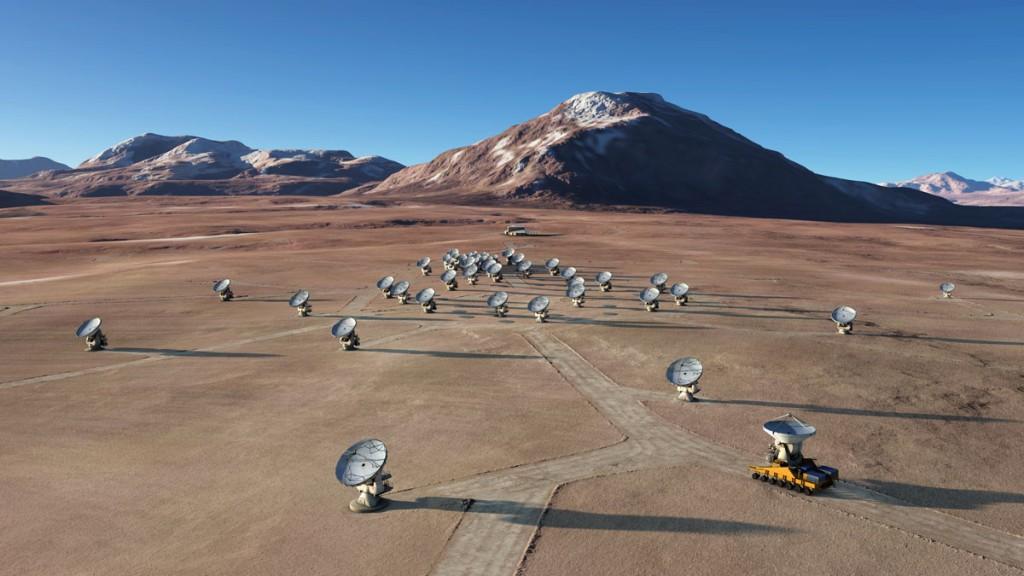
\includegraphics[width=11cm,height=8cm]{images/alma.jpg}
% \caption{ALMA dishes in Atacama Desert}
% \end{figure}


ALMA is an instrument that consists of a giant array of 12-m antennas with baselines up to 16 km, and an additional compact array of 7-m and 12-m antennas to greatly enhance ALMA's ability to image extended targets, located on the Chajnantor plateau at 5000m altitude. Initially, it will observe at wavelengths in the range $3 mm$ to $400 μm$ ($84$ to $720 GHz$). The antennas can be moved around, in order to form arrays with different distributions of baseline lengths. More extended arrays will give high spatial resolution, more compact arrays give better sensitivity for extended sources. In addition to the array of 12-m antennas, there is the Atacama Compact Array (ACA), consisting of twelve 7-m antennas and four 12-m antennas. This array will mostly stay in a fixed configuration and is used to image large scale structures that are not well sampled by the ALMA 12-m array. \newline

The design of ALMA is driven by three key science goals:

\begin{itemize}

\item The ability to detect spectral line emission from CO in a normal galaxy like the Milky Way at a redshift of $z=3$, in less than 24 hours

\item The ability to image the gas kinematics in protostars and in protoplanetary disks around young Sun-like stars in the nearest molecular clouds ($150 pc$)

\item The ability to provide precise high dynamic range images at an angular resolution of $0.1 arcsec$
\end{itemize}
 
ALMA delivers data cubes, of which the third axis is frequency. In this sense, the final data products are very much like that of an integral field unit with up to a million Spectral Pixels. \newline

As stated in \cite{Etoka12}, the purpose of the ALMA archive is to provide services for:

\begin{itemize}
\item Persistent archiving and retrieval for observational data.
\item Observaction descriptors.
\item Datacubes produced by pipeline.
\item Technical and environmental data.
\end{itemize}

And the key-point of the conceptual design of the ALMA Archive is to guarantee that three ALMA Regional Centres (ARCs) hold an identical copy of the archive at the Joint ALMA Observatory (JAO) in Santiago. 

Relational denormalized database.

ALMA front-end archive is optimized for storage and preservation, not for data query and retrieval. ASA database is inspired from ObsCore, RADAMS and Hubble Legacy Archive plus Virtual Observatory Software:

\begin{itemize}
\item openCADC, which is used for database access and VO access protocol
\item VOView, for Web components
\end{itemize}




\section{Square Kilometer Array}

Thousands of linked radio wave receptors will be located in Australia and in Southern Africa. Combining the signals from the antennas in each region will create a telescope with a collecting area equivalent to a dish with an area of about one square kilometer.  \newline

The Square Kilometer Array (SKA) will address fundamental unanswered questions about our Universe including how the first stars and galaxies formed after the Big Bang, how galaxies have evolved since then, the role of magnetism in the cosmos, the nature of gravity, and the search for life beyond Earth.  \newline

The SKA is a global science and engineering project led by the SKA Organisation, a not-for-profit company with its headquarters at Jodrell Bank Observatory, near Manchester.  \newline

An array of dish receptors will extend into eight African countries from a central core region in the Karoo desert of South Africa. A further array of mid frequency aperture arrays will also be built in the Karoo. A smaller array of dish receptors and an array of low frequency aperture arrays will be located in the Murchison Radio-astronomy Observatory in Western Australia. \newline

Construction is scheduled to start in 2016.

% \begin{figure}[H]
% \centering
% 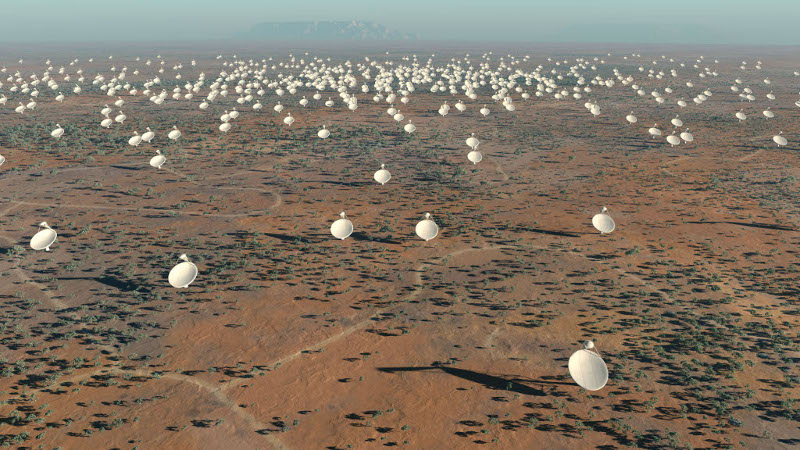
\includegraphics[width=11cm,height=8cm]{images/ska.jpg}
% \caption{Artist's impression of the SKA dishes. Credit: SKA Organisation/TDP/DRAO/Swinburne Astronomy Productions}
% \end{figure}

%\subsection{Figures and facts}

The recent launch of the Murchison Widefield Array (MWA) - a radio telescope based in Western Australia's Mid West - marked the start of an impressive flow of astronomical data that will be stored in the iVEC-managed Pawsey Center in Kensington. \newline

According to Professor Andreas Wicenec, from The University of Western Australia node of the International Centre for Radio Astronomy Research (ICRAR), SKA has ``now have more than 400 megabytes per second of MWA data streaming along the National Broadband Network from the desert 800 km away''. \footnote{\url{http://www.skatelescope.org/news/pawsey-centre/}}  \newline

The Murchison Widefield Array is the first Square Kilometre Array precursor to enter full operations, generating a vast torrent of information that needs to be stored for later retrieval by researchers. \newline

According to Proffesor Wicenec, ``To store the Big Data the MWA produces, you’d need almost three 1 TB hard drives every two hours. The technical challenge isn't just in saving the observations but how you then distribute them to astronomers from the MWA team in far-flung places so they can start using it''.

There are currently two links between the data stores in Perth and MWA researchers at the Massachusetts Institute of Technology (MIT) in the United States and the Victoria University of Wellington in New Zealand. A future link to India -another MWA partner- will also be created. \newline

The data are not obviously intended to be fully available for everybody at every time: for instance, MIT researchers are interested in the early universe so filtering techniques to control what data is copied from the Pawsey Center archive to the MIT machines are used. By 2013, more than 150 TB of data had been transferred automatically to the MIT store, with a stream of up to 4 TB a day increasing that value. \newline

MWA is producing so much information that it would be impossible to manually decide where to send what, which is where a sophisticated archiving system — the open-source Next Generation Archive System (NGAS) — comes in. NGAS was initially developed by Professor Wicenec at the European Southern Observatory (ESO) and later modified by the ICRAR team to meet the MWA data challenge. \newline

In the NGAS one simply asks the system for what the data wanted and it either provides it from the local store or retrieves it from the full archive back in Perth. \newline

About half of all MWA computing occurs on site in the Murchison, where signals from radio telescope antennas are combined and processed in a powerful system of computers called a correlator. What's left to do in Perth is produce images, and manage storage and distribution by the archive system so MWA astronomers can analyze the collected data. Data travels down a dedicated 10 gigabit per second connection between the Murchison Radio-astronomy Observatory (MRO) and Geraldton, and the trip to Perth is completed on Australia’s new high-speed National Broadband Network. \newline

The MWA will store about 3 Petabytes at the Pawsey Center each year. Another section of the Pawsey Center will be a supercomputing facility that includes computing for Australia's other SKA precursor, CSIRO’s Australian Square Kilometre Array Pathfinder (ASKAP), and projects from geoscience and other computationally intensive fields. \newline

To sum up, some relevant figures and facts about SKA:

\begin{itemize}

\item The data collected by the SKA in a single day would take nearly two million years to playback on an ipod.
\item The SKA central computer will have the processing power of about one hundred million PCs.
\item The SKA will use enough optical fibre to wrap twice around the Earth.
\item The dishes of the SKA will produce 10 times the global internet traffic.
\item The SKA will generate enough raw data to fill 15 million 64 GB iPods every day.
\item SKA will be able to detect an airport radar on a planet 50 light years away.

\end{itemize}



\section{Large Synoptic Survey Telescope}

The Large Synoptic Survey Telescope (LSST) is a new kind of telescope whose wide field of view allows it to observe large areas of the sky at once. Taking more than 800 panoramic images each night, it can cover the sky twice each week. Data from LSST will be used to create a 3D map of the Universe with unprecedented depth and detail. This map can be used to locate the mysterious dark matter and to characterize the properties of the even more mysterious dark energy. Plans for sharing the data from LSST with the public are as ambitious as the telescope itself. Anyone with a computer will be able to fly through the Universe, zooming past objects a hundred million times fainter than can be observed with the unaided eye. The work on the project is broken down into three main areas: The Camera, Telescope and Site, and Data Management. \newline

LSST observing will produce about 30 TB per night, leading to a total database over the ten years of operations of 60 PB for the raw data, and 30 PB for the catalog database, that will be processed using 100 TFlops. The data will be sent over existing optical fiber links from South America to the U.S. \newline

Some of the institutional members are Google, Caltech, Harvard-Smithsonian Center for Astrophysics, Fermi National Accelerator Laboratory or STSI. \footnote{For a full list of institutional members, browse to \url{http://lsst.org/lsst/about/members}}  \newline

Currently finishing the design and development stages, it is expected to start operating in 2022.